\documentclass[a4paper,twoside]{scrbook}
\usepackage{CJKutf8}
\usepackage{url}
\usepackage{biblatex}
\usepackage{hyperref}
\usepackage{graphicx}
\addbibresource{v1pc.bib}
\begin{document}
\begin{CJK}{UTF8}{gbsn}
\title{Volume 1, Part C: Early Memory Model}
\author{EDI}

\frontmatter
\maketitle
\tableofcontents
\mainmatter

\chapter{Introduction}
\section{Collective Communications Library}
\subsection{NVIDIA Collective Communications Library(NCCL)}
1991年,Argonne 国家实验室、Cornell 大学、MIT、Oak Ridge 国家实验室和 Wisconsin 大学联合成立了 MPI 论坛\cite{mpiforum},旨在制定一个标准化的消息传递接口。1994 年,MPI 论坛发布了第一个 MPI 标准版本 1.0,该版本定义了 120 个函数,涵盖了点对点通信、集合通信、进程管理、数据类型操作和错误处理等功能。MPI不受任何主要标准机构的认可,但是它已成为对在分布式内存系统上运行的并行程序进行建模的进程之间通信的事实标准。随着并行计算需求的不断扩大,MPI不断演进至今已经发布了MPI 4.1版本。

2016年,NVIDIA研究员Nathan Luehr发现在实践中,多GPU环境下并行计算的效率并没有像理论分析的那样获得显著提升,原因是多GPU环境下处理器的利用率低以及处理器的数据交换占据了大量的计算时间。为了充分利用GPU间的带宽,Nathan Luehr提出了NVIDIA Collective Communications Library(NCCL)]\cite{nccl2016},NCCL是一个通信原语库,具备拓扑感知,构造了基于环的消息通知路径。对于连接在同一个PCIe总线上的GPU,NCCL可以很好地促进GPU带宽的利用,从而使得小部分的线程通信和大部分的线程计算能够同时进行。不过,NCCL只适用于单节点环境,虽然对于单节点内的GPU数量没有限制,但是对于混用不同型号的GPU处理效果不好。

2016年,A. A. Awan\cite{awan2016}等人针对高性能数据分析 (HPDA) 和深度学习 (DL) 等新兴应用对高性能计算 (HPC) 平台和编程框架的挑战,提出了一种高效的 MPI\_Bcast设计,用于在多 GPU 节点之间进行大规模 GPU 缓冲区通信,同时利用NCCL库高效地进行节点内地通信。实验结果表明,与现有的 MVAPICH2-GDR 实现相比,所提出的分层 MPI\_Bcast 设计可以将 CNTK 框架的训练时间提高高达 47\%。不过,该算法依赖于 NCCL 库和 MVAPICH2-GDR 运行时。这意味着算法只能在支持这些组件的系统上运行。对于不支持 NCCL 库或 MVAPICH2-GDR 运行时的系统,需要寻找其他方法来实现高效的大规模 GPU 通信。

2018年,Iman Faraji\cite{cpe4667}等人讨论了在MPI中进行GPU集体通信的优化方法,为了将GPU感知引入MPI集体通信,提出了GPU共享缓冲区感知(GSB)算法和二叉树(BTB)算法。设计了用于多GPU节点的分层框架,并将其用于(1) intra-node intra-GPU、(2) intra-node inter-GPU、(3) inter-node inter-GPU。在单GPU节点中,作者通过GSB和BTB来最小化集体通信中消息的大小,利用GPU共享缓冲区和CUDA进程间通信支持MPI进程之间的GPU通信。在多GPU节点中,作者组合GSB—BTB算法,结合MVAPICH2进行全局操作提高集体通信性能。
\subsection{Microsoft Collective Communication Language(MSCCLang)}
2023年,Aashaka Shah\cite{shah2023taccl}等人提出opology Aware Col-lective Communication Library(TACCL)。针对不同拓扑结构需要重新单独设计算法的问题,TACCL引入了通信草图概念,包含逻辑拓扑、交换机超边策略、算法对称性和输入大小等信息,允许算法设计师只考虑顶层设计而不用实施底层实现。相比于NCCL,TACCL在多个集合通信操作和硬件拓扑上都展现出了优势,比NCCL快1.7-6。7不等。

2023年,Meghan Cowan\cite{cowan2023mscclang}等人提出了Microsoft Collective Communication Language(MSCCLang),旨在解决大规模机器学习模型在多 GPU 系统上训练和推理时,集体通信成为瓶颈的问题。它包含一个领域特定语言(DSL)用于编写集体通信算法,以及一个优化编译器,将算法转换为可执行的代码,并能够在基于解释器的运行时环境中高效灵活地执行。
\section{Remote Procedure Call}
本章节参考了\href{https://cloud.tencent.com/developer/article/1619589}{RPC发展史}

这里提及的远程过程调用(Remote Procedure Call,RPC)是广义上远程调用手段,是一种允许两个实体通过通用请求/响应机制的通信通道进行通信的设计范例,包括RPC(remote procedure call,远程过程调用)、SOAP(simple object access protoal,简单对象访问协议)、REST(representational state transfer,表达性状态转移)等设计范例。

1984年,Birrell\cite{birrell1984implementing}等人在《Implementing remote procedure calls》中对RPC做了最经典的解释。作者阐述了RPC传输协议的设计目标,描述了简单调用、复杂调用、异常处理、性能优化等问题,如图\ref{fig:A simple call}所示,文章给出了一次调用的实例图,用户代码通过本地调用请求 RPC,将参数传递给用户存根。用户存根将参数打包成调用数据包,并将其发送给 RPC 运行时。RPC 运行时负责将调用数据包可靠地传输到被调用方机器。
\begin{figure}[!htbp]
\centering
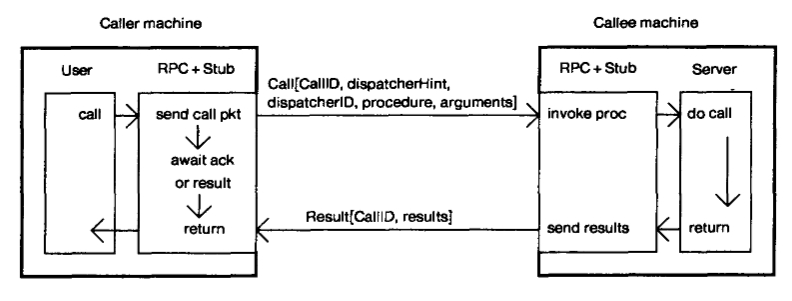
\includegraphics[width=1\textwidth]{Figures/A simple call.png}
\caption{一次调用过程} 
\label{fig:A simple call}
\end{figure}
1988年,RFC 1057 发布,ONC RPC 被定义为标准的RPC 规范,ONC RPC 提供了一个编译器,需要一个远程过程接口的定义来生成客户端和服务器的存根函数。这个编译器叫做 rpcgen。在运行此编译器之前,程序员必须提供接口定义。包含函数声明的接口定义,通过版本号进行分组,并被一个独特的程序编码来标识。该程序编码能够让客户来确定所需的接口。版本号是非常有用的,即使客户没有更新到最新的代码仍然可以连接到一个新的服务器,只要该服务器还支持旧接口。
\subsection{Common Object Request Broker Architecture(CORBA)}
分布式计算与面向对象编程的结合催生了分布式对象中间件,OMG在此需求的基础上提出了CORBA。CORBA是面向对象的应用程序体系规范,为用户提供接口定义语言(IDL)来指定远程对象类接口。用户的请求以对象代理请求(ORB)的方式处理,ORB截取客户发送的请求,并负责在该软件总线上找到实现该请求的服务对象,然后完成参数、方法调用,并返回最终结果。自OMG提出CORBA之后,CORBA经过了一段时间的黄金期,但是还是因为各种因素逐渐退出了历史舞台。下文详细分析了CORBA经历的早期发展、中期挑战、后期衰落以及发展现状等内容\cite{siegel1998omg} \cite{henning2006rise}。

(1)早期发展 (上世纪90年代初):1991年, OMG提出了CORBA1.0,用于帮助开发人员构建异构分布式应用。CORBA为用户提供了 IDL (接口定义语言),用于定义对象接口的标准语言,确保不同编程语言之间的互操作性;ORB (对象请求代理),管理对象调用和通信,隐藏底层细节,简化开发;IIOP (互联网ORB协议),标准的网络通信协议,确保跨网络传输的互操作性。得益于其强大的互操作性、成熟的分布式计算模型、丰富的标准服务以及广泛的应用成功案例,使其成为构建大型企业级应用的首选技术之一。

(2)中期挑战 (上世纪90年代中后期):1996年,添加了几个主要功能,包括用于客户端可移植性扩展的动态骨架接口(动态调用的镜像),初始参考解析器到接口库“开箱即用”互操作体系结构(GIOP、IIOP®、DCE-CIOP),支持COBOL的分层安全和事务服务数据类型扩展、科学处理、与OLE2/COM的宽字符互操作。OMG发布CORBA2.0,不过,CORBA2.0的推广并不顺利,Java 和 Web 开始兴起,虽然CORBA提供了Java语言映射,但是并没有涉及到爆炸式增长的Web。商业公司并没有等待CORBA给出解决方案,它们转向了其它技术,并且开始构建他们基于Web浏览器、HTTP、Java和EJB的电子商务基础设施。

(3)后期衰落 (2000年初): 2000年初,互联网泡沫破裂,XML 和 Web 服务兴起,进一步削弱 CORBA 的市场地位。CORBA的衰落是有原因的,可以分为技术上的复杂性和组织流程上的失败。
技术问题:

API的复杂性: API 复杂且难以使用,架构选择不当,类型系统过于庞大。

安全功能不足: 缺乏安全性和版本控制机制。

其他技术问题: 互操作性协议设计缺陷,编码冗余,缺乏对线程和异步调用的支持等。

上述的技术问题带来的结果就是,CORBA学习曲线陡峭,技术复杂,不容易正确使用,这些因素导致开发周期长、易出错。早期的实现常常充满Bug并且缺乏有质量的文档,有经验的CORBA程序员稀缺。

流程问题:

OMG是一个基于成员一致同意来发布技术的组织。从根本上来说,成员通过投票来将意见征求书变成规范。成员公司提交草案规范作为回应,OMG的成员们通过投票来决定是否将提案接受为标准。理论上,这是一个民主、公平的过程,但是实际上,它并不能起作用。标准化过程中没有什么准入资格。一些贡献者是领域专家,但是,令人感到挫折的是,大量的成员几乎不理解他们所要投票的技术,并且参与投票的厂商之间存在利益冲突。

缺乏对现有最佳实践的标准化,以及对参考实现和实际应用项目的需求,导致技术不成熟和难以使用。

(4)现状: CORBA 主要用于企业内部网络和实时嵌入式系统开发,已沦为垂直领域的细分技术。

\subsection{XML-RPC}
SOAP是一种建立在XML上的通信协议。

1998 年 XML 1.0 发布,被 W3C (World Wide Web Consortium) 推荐为标准的描述语言。同年,微软和DevelopMentor发布SOAP(Simple Object Access Protocol),随后提交给W3C作为标准。SOAP是一个严格定义的信息交换协议,使用XML作为RPC新的对象序列化机制,用于在Web Service中把远程调用和返回封装成机器可读的格式化数据。SOAP 的服务发现用的是 UDDI(Universal Description, Discovery, Integration) 统一描述发现集成,相当于一个注册中心,服务提供方将 WSDL 文件发布到注册中心,使用方可以到这个注册中心查找。

SOAP严格意义上是属于XML-RPC(XML Remote Procedure Call)技术的一个变种,一个XML-RPC请求消息就是一个HTTP-POST请求消息,其请求消息主体基于XML格式。客户端发送XML-RPC请求消息到服务端,调用服务端的远程方法并在服务端上运行远程方法。远程方法执行完毕后返回响应消息给客户端,其响应消息主体同样基于XML格式。远程方法的参数支持数字、字符串、日期等,也支持列表数组和其他复杂结构类型,SOAP是第一次真正成功地解决了多语言多平台支持的开放性RPC标准。
\subsection{RESTful API}
Restful是一种基于HTTP的架构设计风格。

2000年,Roy Thomas Fielding在《Architectural Styles and the Design of Network-based Software Architectures》\cite{fielding2000architectural}中首次提出了REST架构,直到目前仍然是Web开发的主流架构设计风格。REST架构风格定义了六个指导性约束。
\subsubsection{客户端-服务器架构}
通过将用户界面问题与数据存储问题分开,提高了跨多个平台的用户界面的可移植性,并通过简化服务器组件提高了可扩展性。
\subsubsection{统一接口}
统一接口是一切 RESTful Web 服务设计的基础。其表示服务器以标准格式传输信息。格式化的资源在 REST 中称为表征。此格式可以与服务器应用程序上资源的内部表征不同。例如,服务器可以将数据存储为文本,但以 HTML 表征格式发送该数据。

统一接口强制实施四个架构约束:

(1)请求应确定资源,它们通过使用统一的资源标识符实现此功能。

(2)客户端包含资源表征中的足够信息以修改或删除资源(如需要),服务器通过发送进一步描述资源的元数据以符合这一条件。

(3)客户端接收有关如何进一步处理表征的信息,服务器通过发送自描述信息实现此功能,该信息包含了有关客户端如何以最佳方式使用这些信息的元数据。

(4)客户端接收有关其完成任务需要的所有其他相关资源的信息,服务器通过在表征中发送超链接实现此功能,以便客户端可以动态发现更多资源。
\subsubsection{无状态}
在 REST 架构中,无状态指一种服务器独立于所有之前的请求完成每个客户端请求的通信方法。客户端可以以任意顺序请求资源,每个请求为无状态或与独立于其他请求。此 REST API 设计约束意味着服务器每次可以完全识别和满足请求。 
\subsubsection{层次化系统}
在层次化系统架构中,客户端可以连接到客户端和服务器之间的其他授权中间方,其仍将接收来自服务器的响应。服务器也可以将请求传递到其他服务器。您可以将 RESTful Web 服务设计为在包含多个层级(例如安全、应用程序和业务逻辑)的数个服务器上运行,从而共同满足客户端请求。这些层级对客户端仍不可见。
\subsubsection{高速缓存能力}
RESTful Web 服务支持缓存,缓存是指将一些响应存储在客户端或中间方上以提高服务器响应时间的流程。例如,假设您访问某个网站,该网站的每个页面都包含通用的页眉和页脚图像。每次您访问新的网站页面时,服务器必须重新发送相同的图像。为了避免出现这种情况,客户端在首次响应后会缓存或存储这些图像,之后直接使用缓存中的图像。RESTful Web 服务通过使用自行定义为可缓存或不可缓存的 API 响应来控制缓存。
\subsubsection{按需编码}
在 REST 架构风格中,服务器可以通过将软件编程代码传输到客户端暂时扩展或自定义客户端功能。例如,当您在任何网站上填写注册表单时,浏览器会立即高亮您填写内容的任何错误,例如不正确的电话号码。正是由于服务器发送的代码,浏览器才可以实现这个功能。
\subsection{微服务架构}
随着互联网数据的指数式增长,微服务架构开始出现并普及,分布式系统开始变的无处不在,REST架构的缺点开始显现,基于JSON或者XML 的消息冗余严重,导致性能下降。

2008年,Google 开源 Protocol Buffer,这是一种轻便高效的结构化数据存储格式,可以用于结构化数据序列化,很适合做数据存储或 RPC 数据交换格式。它可用于通讯协议、数据存储等领域的语言无关、平台无关、可扩展的序列化结构数据格式。

2008年,FaceBook 开源 thrift,这是一个跨语言的服务部署框架,最初由Facebook于2007年开发,2008年进入Apache开源项目。Thrift通过一个中间语言(IDL, 接口定义语言)来定义RPC的接口和数据类型,然后通过一个编译器生成不同语言的代码(目前支持C++,Java, Python, PHP, Ruby, Erlang, Perl, Haskell, C\#, Cocoa, Smalltalk和OCaml),并由生成的代码负责RPC协议层和传输层的实现。

2010年,Avro脱离Hadoop项目,成为Apache顶级项目。这是一个基于二进制数据传输高性能的中间件。在Hadoop的其他项目中例如HBase(Ref)和Hive(Ref)的Client端与服务端的数据传输也采用了这个工具。Avro 可以将数据结构或对象转化成便于存储或传输的格式。

2015年,Google 开源Google Remote Procedure Cal(gRPC),gRPC 使用 PB 作为序列化的解决方案,而在传输的介质上使用了 HTTP/2而不是常见的TCP。gRPC 是一个多路复用、双向流式 RPC 协议。在一般的 RPC 机制中,客户端发起到服务器的连接,只有客户端可以请求,而服务器只能响应传入的请求。然而,在双向 gRPC 流中,虽然初始连接是由客户端发起的(称为端点1) ,但是一旦建立连接,服务器(称为端点2)和端点1都可以发送请求和接收响应。这极大地简化了两个端点相互通信的开发(如网格计算)。由于两个数据流都是独立的,这也省去了在端点之间创建两个独立连接的麻烦(一个从端点1到端点2,另一个从端点2到端点1)。

\section{Consensus Mechanism}
\subsection{Byzantine fault-tolerant(BFT)}
BFT自20世纪80年代提出以来\cite{lamport1982byzantine},已经得到了广泛的研究。在第一个被称为PBFT\cite{castro2002practical}的实用BFT协议之后,有许多实用BFT协议被提出。根据时序假设,BFT可以分为三种类型:同步、异步和部分同步协议。

2016年,Andrew Miller等人提出了HoneyBadgerBFT\cite{miller2016honey},这是第一个实用的异步BFT协议,它在不做任何时序假设的情况下保证了生存性。HoneyBadgerBFT的核心部分由两部分组成,分别是原子广播(Atomic Broadcast)和异步公共子集协议(Asynchronous Common Subset),在协议开始以前,每个主机准备好各自的提案(即试图写入共识的数据),启动N个原子广播的实例(N为网络中主机的个数)。在某一个原子广播完成以后遂将该广播对应的主机编号作为输入启动异步公共子集协议。异步公共子集协议在收集到足够多的主机编号后终止,所有的非敌手主机得到一个关于子集的共识。根据这个子集这些主机将从原子广播阶段获得的提案写入共识。

2017年,Yossi Gilad\cite{gilad2017algorand}等人在针对 PBFT 算法在很多节点情况下性能不佳的问题,提出先选出少量记账节点,然后再利用可验证随机函数(Verifiable Random Function,VRF)来随机选取领导节点,避免全网直接做共识,将拜占庭算法扩展到了支持较大规模的应用场景,同时保持较好的性能(1000+ tps)。

同年,Rafael Pass \cite{pass2017sleepy}等人探讨了在动态场景(大量节点离线情况)下如何保障共识的安全性,提出的 Sleepy Consensus 算法可以在活跃诚实节点达到一半以上时确保完成拜占庭共识。

2019年,Maofan Yin 等在论文《HotStuff: BFT Consensus with Linearity and Responsiveness》\cite{yin2019hotstuff}中对 PBFT 算法进行了改进:利用主节点来简化通信量,同时将视图切换与共识操作进行统一。值得一提的是,Facebook Libra 白皮书中采用了该成果。

\subsection{Consensus mechanism based on proof of concepts}
由于无许可的区块链网络不允许身份验证或显式同步方案。因此,期望其中的共识协议具有良好的可扩展性,并且能够容忍伪身份和较差的同步。由于任何节点都能够为区块链头部提出具有自己的候选块的状态转换,因此无许可网络中的共识协议的主要目标是确保每个共识节点都遵守“最长链规则”[3]。也就是说,当块被组织在链表中时,在任何时间实例中,只有最长的链可以被接受为区块链的规范状态。由于缺乏身份验证,基于直接投票的BFT协议不适合无许可的区块链网络。基于激励的Nakamoto Consensus\cite{nakamoto2008bitcoin}被广泛采用。

在Nakamoto Consensus的基础下,产生了许多基于概念证明的共识机制,包括PoW、
PoUS、uPoW、PoR、PoST、PoM、PoH等方案。

\subsection{Virtual Block Mining and Hybrid Consensus Mechanisms Beyond Proof of Concept}
2019年,Wenbo Wang等人在《A Survey on Consensus Mechanisms and Mining Strategy Management in Blockchain Networks》\cite{wang2019survey}对超越概念证明的虚拟块挖掘和混合共识机制进行了讨论,文中提出了两种类型:基于股权证明和虚拟挖矿和混合共识协议。

在基于股权证明和虚拟挖矿中,介绍了PoS的概念,它是一种修改后的PoW方案,旨在减少因耗尽哈希查询而产生的能源消耗。讨论了纯PoS协议的设计,例如Ouroboros协议,它使用“跟随硬币”算法来选举区块提议的领导者,并根据持有者的股份进行随机分配。讨论了基于委员会的PoS协议,例如PoA和Snow White协议,它们将领导者选举和区块生成/验证过程结合在一起,类似于传统的拜占庭容错协议。

=======
在混合共识协议中,讨论了将Nakamoto协议与快速拜占庭容错协议(如BFT)结合起来的方法,以实现更高的吞吐量和立即的最终性。介绍了Bitcoin-NG协议,它将共识过程分解为领导者选举和事务序列化两个平面,并使用两种类型的区块来实现更高的吞吐量。讨论了PeerCensus协议,它使用PoW方案来选择BFT委员会成员,并确保事务提交与区块生成独立进行。讨论了将虚拟挖矿机制(如PoS)与BFT协议结合起来的方法,例如Tendermint协议,它使用股份来衡量投票权,并通过轮询方案来选择区块提议的领导者。
\printbibliography
\end{CJK}
\end{document}
